\documentclass[14pt]{extbook}
\usepackage{multicol, enumerate, enumitem, hyperref, color, soul, setspace, parskip, fancyhdr} %General Packages
\usepackage{amssymb, amsthm, amsmath, bbm, latexsym, units, mathtools} %Math Packages
\everymath{\displaystyle} %All math in Display Style
% Packages with additional options
\usepackage[headsep=0.5cm,headheight=12pt, left=1 in,right= 1 in,top= 1 in,bottom= 1 in]{geometry}
\usepackage[usenames,dvipsnames]{xcolor}
\usepackage{dashrule}  % Package to use the command below to create lines between items
\newcommand{\litem}[1]{\item#1\hspace*{-1cm}\rule{\textwidth}{0.4pt}}
\pagestyle{fancy}
\lhead{Progress Quiz 3}
\chead{}
\rhead{Version C}
\lfoot{}
\cfoot{}
\rfoot{Fall 2020}
\begin{document}

\begin{enumerate}
\litem{
Factor the quadratic below. Then, choose the intervals that contain the constants in the form $(ax+b)(cx+d); b \leq d.$\[ 54x^{2} -15 x -25 \]\begin{enumerate}[label=\Alph*.]
\item \( a \in [1.54, 2.3], \hspace*{5mm} b \in [-6, -3], \hspace*{5mm} c \in [26.6, 27.9], \text{ and } \hspace*{5mm} d \in [0, 6] \)
\item \( a \in [-0.19, 1.84], \hspace*{5mm} b \in [-51, -43], \hspace*{5mm} c \in [0.6, 1.8], \text{ and } \hspace*{5mm} d \in [22, 34] \)
\item \( a \in [17.45, 18.5], \hspace*{5mm} b \in [-6, -3], \hspace*{5mm} c \in [2.5, 3.2], \text{ and } \hspace*{5mm} d \in [0, 6] \)
\item \( a \in [4.96, 7.25], \hspace*{5mm} b \in [-6, -3], \hspace*{5mm} c \in [8.6, 10.3], \text{ and } \hspace*{5mm} d \in [0, 6] \)
\item \( \text{None of the above.} \)

\end{enumerate} }
\litem{
Graph the equation below.\[ f(x) = (x+1)^2 + 18 \]\begin{enumerate}[label=\Alph*.]
\begin{multicols}{2}\item 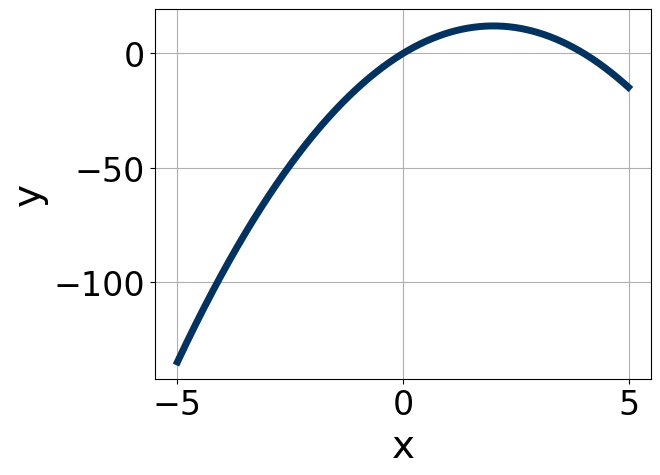
\includegraphics[width = 0.3\textwidth]{../Figures/quadraticEquationToGraphAC.png}\item 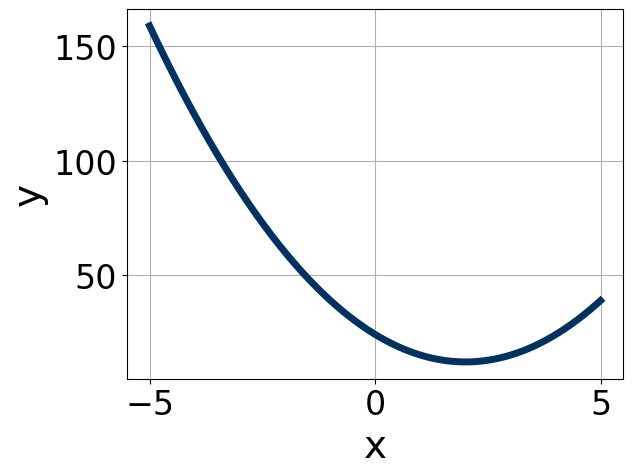
\includegraphics[width = 0.3\textwidth]{../Figures/quadraticEquationToGraphBC.png}\item 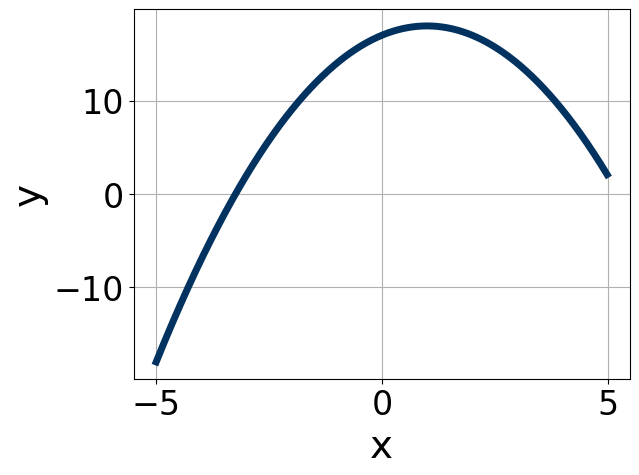
\includegraphics[width = 0.3\textwidth]{../Figures/quadraticEquationToGraphCC.png}\item 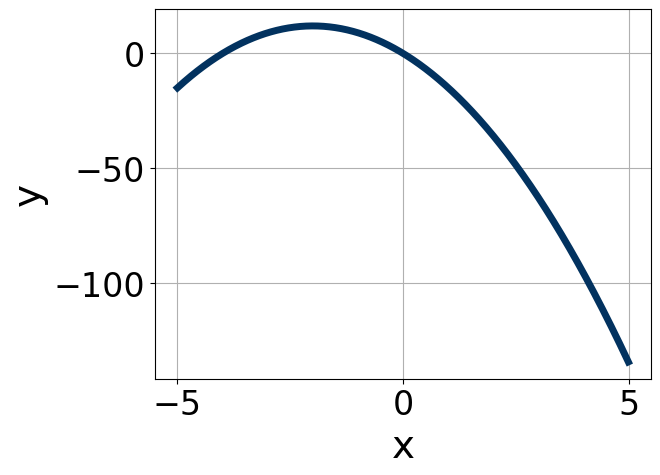
\includegraphics[width = 0.3\textwidth]{../Figures/quadraticEquationToGraphDC.png}\end{multicols}\item None of the above.
\end{enumerate} }
\litem{
Write the equation of the graph presented below in the form $f(x)=ax^2+bx+c$, assuming  $a=1$ or $a=-1$. Then, choose the intervals that $a, b,$ and $c$ belong to.
\begin{center}
    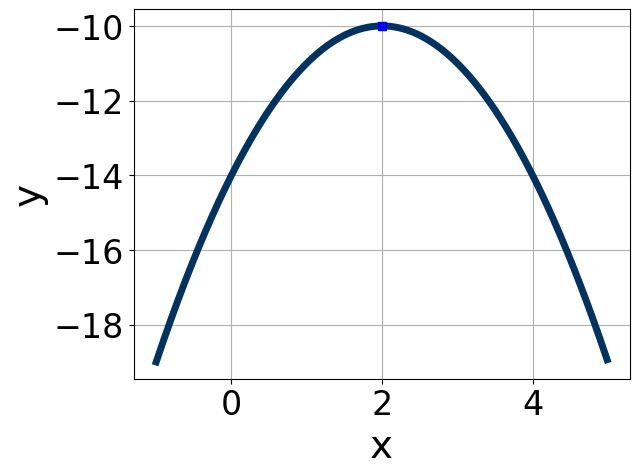
\includegraphics[width=0.5\textwidth]{../Figures/quadraticGraphToEquationC.png}
\end{center}
\begin{enumerate}[label=\Alph*.]
\item \( a \in [0.1, 2.3], \hspace*{5mm} b \in [-8, -2], \text{ and } \hspace*{5mm} c \in [-7, -5] \)
\item \( a \in [-1.9, -0.5], \hspace*{5mm} b \in [-8, -2], \text{ and } \hspace*{5mm} c \in [3, 7] \)
\item \( a \in [-1.9, -0.5], \hspace*{5mm} b \in [-8, -2], \text{ and } \hspace*{5mm} c \in [-18, -9] \)
\item \( a \in [0.1, 2.3], \hspace*{5mm} b \in [2, 8], \text{ and } \hspace*{5mm} c \in [-7, -5] \)
\item \( a \in [-1.9, -0.5], \hspace*{5mm} b \in [2, 8], \text{ and } \hspace*{5mm} c \in [-18, -9] \)

\end{enumerate} }
\litem{
Solve the quadratic equation below. Then, choose the intervals that the solutions $x_1$ and $x_2$ belong to, with $x_1 \leq x_2$.\[ 10x^{2} +57 x + 54 = 0 \]\begin{enumerate}[label=\Alph*.]
\item \( x_1 \in [-45.2, -44.55] \text{ and } x_2 \in [-12.27, -11.72] \)
\item \( x_1 \in [-4.62, -3.84] \text{ and } x_2 \in [-1.33, -0.89] \)
\item \( x_1 \in [-4.29, -3.47] \text{ and } x_2 \in [-1.73, -1.44] \)
\item \( x_1 \in [-9.32, -8.81] \text{ and } x_2 \in [-0.76, -0.54] \)
\item \( x_1 \in [-14.29, -13.16] \text{ and } x_2 \in [-0.56, -0.26] \)

\end{enumerate} }
\litem{
Factor the quadratic below. Then, choose the intervals that contain the constants in the form $(ax+b)(cx+d); b \leq d.$\[ 54x^{2} +33 x -10 \]\begin{enumerate}[label=\Alph*.]
\item \( a \in [17.3, 19.7], \hspace*{5mm} b \in [-6, 0], \hspace*{5mm} c \in [1.6, 4.3], \text{ and } \hspace*{5mm} d \in [5, 7] \)
\item \( a \in [2.4, 4.6], \hspace*{5mm} b \in [-6, 0], \hspace*{5mm} c \in [15.6, 19.4], \text{ and } \hspace*{5mm} d \in [5, 7] \)
\item \( a \in [-1.1, 1.4], \hspace*{5mm} b \in [-15, -11], \hspace*{5mm} c \in [-3.3, 1.9], \text{ and } \hspace*{5mm} d \in [44, 47] \)
\item \( a \in [6, 11.2], \hspace*{5mm} b \in [-6, 0], \hspace*{5mm} c \in [4.5, 6.3], \text{ and } \hspace*{5mm} d \in [5, 7] \)
\item \( \text{None of the above.} \)

\end{enumerate} }
\litem{
Solve the quadratic equation below. Then, choose the intervals that the solutions belong to, with $x_1 \leq x_2$ (if they exist).\[ -10x^{2} -15 x + 3 = 0 \]\begin{enumerate}[label=\Alph*.]
\item \( x_1 \in [-1.76, -1.44] \text{ and } x_2 \in [-0.09, 0.45] \)
\item \( x_1 \in [-0.23, -0.12] \text{ and } x_2 \in [1.25, 2.17] \)
\item \( x_1 \in [-1.84, -1.71] \text{ and } x_2 \in [16.01, 16.82] \)
\item \( x_1 \in [-19.52, -19.31] \text{ and } x_2 \in [17.46, 18.13] \)
\item \( \text{There are no Real solutions.} \)

\end{enumerate} }
\litem{
Solve the quadratic equation below. Then, choose the intervals that the solutions belong to, with $x_1 \leq x_2$ (if they exist).\[ 13x^{2} +12 x -8 = 0 \]\begin{enumerate}[label=\Alph*.]
\item \( x_1 \in [-0.52, -0.43] \text{ and } x_2 \in [0.8, 2.2] \)
\item \( x_1 \in [-18.45, -17.12] \text{ and } x_2 \in [5.3, 6.3] \)
\item \( x_1 \in [-24.23, -23.46] \text{ and } x_2 \in [22.7, 23.9] \)
\item \( x_1 \in [-1.64, -1.33] \text{ and } x_2 \in [-0.5, 1.2] \)
\item \( \text{There are no Real solutions.} \)

\end{enumerate} }
\litem{
Write the equation of the graph presented below in the form $f(x)=ax^2+bx+c$, assuming  $a=1$ or $a=-1$. Then, choose the intervals that $a, b,$ and $c$ belong to.
\begin{center}
    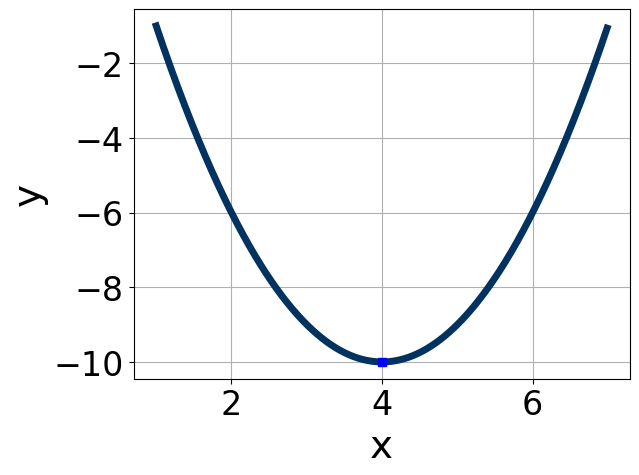
\includegraphics[width=0.5\textwidth]{../Figures/quadraticGraphToEquationCopyC.png}
\end{center}
\begin{enumerate}[label=\Alph*.]
\item \( a \in [1, 3], \hspace*{5mm} b \in [6, 9], \text{ and } \hspace*{5mm} c \in [3, 8] \)
\item \( a \in [1, 3], \hspace*{5mm} b \in [-9, -7], \text{ and } \hspace*{5mm} c \in [3, 8] \)
\item \( a \in [-4, 0], \hspace*{5mm} b \in [-9, -7], \text{ and } \hspace*{5mm} c \in [-28, -22] \)
\item \( a \in [1, 3], \hspace*{5mm} b \in [6, 9], \text{ and } \hspace*{5mm} c \in [24, 30] \)
\item \( a \in [-4, 0], \hspace*{5mm} b \in [6, 9], \text{ and } \hspace*{5mm} c \in [-28, -22] \)

\end{enumerate} }
\litem{
Solve the quadratic equation below. Then, choose the intervals that the solutions $x_1$ and $x_2$ belong to, with $x_1 \leq x_2$.\[ 15x^{2} -32 x + 16 = 0 \]\begin{enumerate}[label=\Alph*.]
\item \( x_1 \in [0.2, 0.3] \text{ and } x_2 \in [3.77, 4.05] \)
\item \( x_1 \in [11.96, 12.08] \text{ and } x_2 \in [19.77, 20.44] \)
\item \( x_1 \in [0.71, 0.83] \text{ and } x_2 \in [0.89, 1.57] \)
\item \( x_1 \in [0.33, 0.45] \text{ and } x_2 \in [2.52, 2.96] \)
\item \( x_1 \in [0.65, 0.74] \text{ and } x_2 \in [1.45, 1.74] \)

\end{enumerate} }
\litem{
Graph the equation below.\[ f(x) = (x+3)^2 + 17 \]\begin{enumerate}[label=\Alph*.]
\begin{multicols}{2}\item 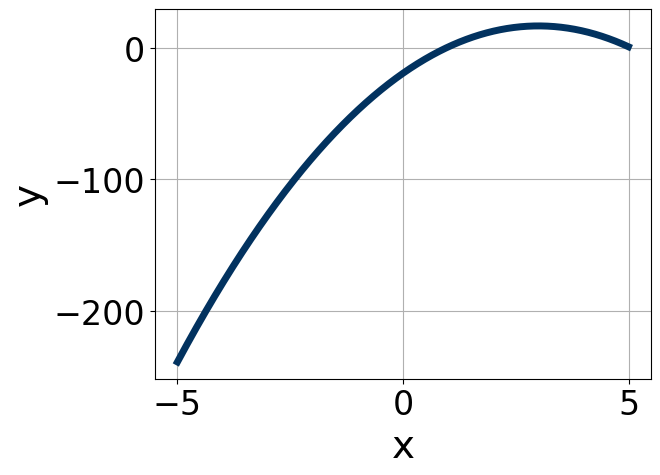
\includegraphics[width = 0.3\textwidth]{../Figures/quadraticEquationToGraphCopyAC.png}\item 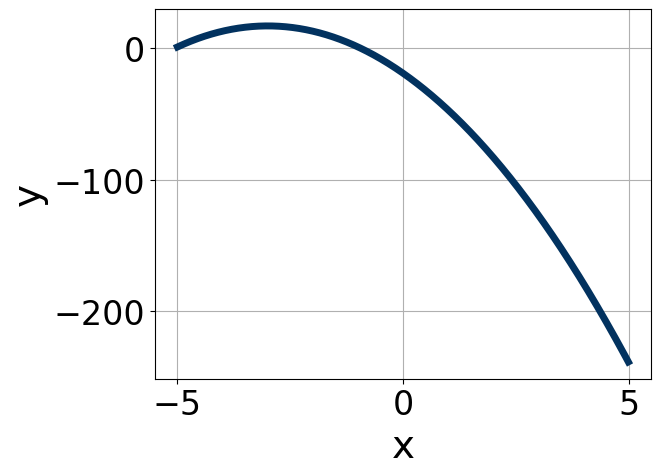
\includegraphics[width = 0.3\textwidth]{../Figures/quadraticEquationToGraphCopyBC.png}\item 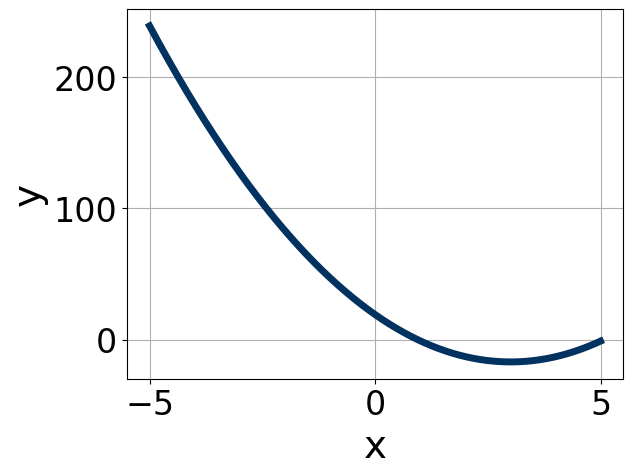
\includegraphics[width = 0.3\textwidth]{../Figures/quadraticEquationToGraphCopyCC.png}\item 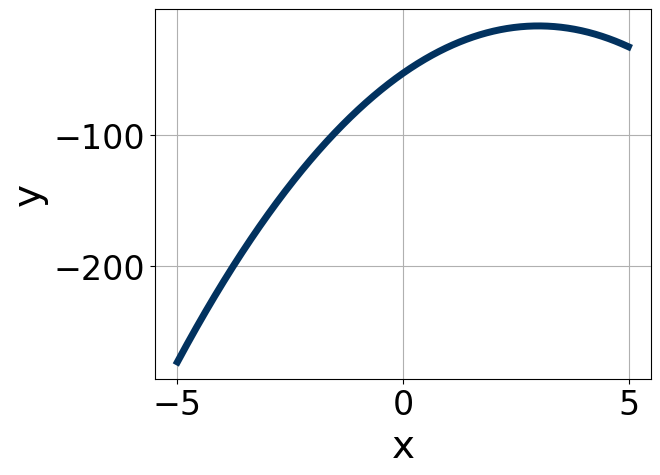
\includegraphics[width = 0.3\textwidth]{../Figures/quadraticEquationToGraphCopyDC.png}\end{multicols}\item None of the above.
\end{enumerate} }
\end{enumerate}

\end{document}